%%%%%%%%%%%%%%%%%%% - TÍTULOS - %%%%%%%%%%%%%%%%%%

\section{TÍTULOS} \label{sec:titulos}

En los documentos de clase \texttt{article} (los distintos tipos de documentos disponibles así como sus diferentes aplicaciones pueden consultarse en \url{https://en.wikibooks.org/wiki/LaTeX/Document_Structure#Document_classes}) existen por defecto tres profundidades de títulos numerados, en orden jerárquico: \texttt{\textbackslash section}, \texttt{\textbackslash subsection} y \texttt{\textbackslash subsubsection}. El título del presente capítulo es un ejemplo de título de profundidad 1 (comando \texttt{\textbackslash section}).


\subsection{Profundidad 2}

Hola que tal. Este es un ejemplo de título de profundidad 2 (comando \texttt{\textbackslash subsection}) que, como se puede ver, queda automáticamente numerado con respecto al título jerárquicamente superior (profundidad 1) inmediatamente anterior.


\subsubsection{Profundidad 3}

Este es un ejemplo de título de profundidad 3 (comando \texttt{\textbackslash subsubsection}) que, de nuevo, se numera automáticamente con respecto al título jerárquicamente superior (profundidad 2) inmediatamente anterior.


\paragraph{Profundidad 4}

En este documento se añade una profundidad de títulos numerados adicional (mediante los comandos \texttt{\textbackslash setcounter\{secnumdepth\}\{4\}} y \texttt{\textbackslash setcounter\{tocdepth\}\{4\}}, ver preámbulo para más información). Así, el comando \texttt{\textbackslash paragraph} se utiliza para incorporar títulos de profundidad 4, como en el caso del título del presente apartado. 

Si se quisiera aumentar en un grado más la profundidad de títulos, bastaría con asignar el valor 5 a ambos comandos \texttt{\textbackslash setcounter} (\texttt{\textbackslash setcounter\{secnumdepth\}\{5\}} y \texttt{\textbackslash setcounter\{tocdepth\} \{5\}}), y realizar los cambios pertinentes en el comando \texttt{\textbackslash subparagraph} de modo que su formato sea coherente con el del resto de títulos (de la misma forma que lo realizado con el comando \texttt{\textbackslash paragraph}, ver preámbulo para más información)


\subsection{Formato y numeración}

La numeración así como el formato de los títulos (tamaño de fuente, tipografía, etc.) utilizados en este documento corresponden a los valores por defecto (excepto en el caso de \texttt{\textbackslash paragraph}, como se explica más arriba), pero pueden ser modificados en el preámbulo del documento (una breve guía sobre la personalización del formato de los títulos puede consultarse en \url{https://www.overleaf.com/learn/latex/sections_and_chapters#Customize_chapters_and_sections}). 

En caso de que no se quiera numerar alguno de los títulos, basta con añadir un asterísco (\textbf{*}) al comando correspondiente, como por ejemplo \texttt{\textbackslash subsection*\{Título sin numerar\}}:


\subsection*{Título sin numerar} 
\addcontentsline{toc}{subsection}{Título sin numerar}

Los títulos sin numerar no aparecen en la tabla de contenidos (índice), pero pueden ser añadidos con ayuda del comando \texttt{\textbackslash addcontentsline\{toc\}} (utilizado previamente para los apartados de Agradecimientos y Resumen ejecutivo), que en este caso quedaría como: \texttt{\textbackslash addcontentsline\{toc\} \ \{subsection\}\{Título sin numerar\}}.


\subsection{Referencias con el comando \texttt{\textbackslash label}} \label{sec:referencias}

Los comandos \texttt{\textbackslash label} se utilizan en \LaTeX \ para colocar referencias que puedan ser utilizadas a lo largo del documento. Son especialmente útiles, como se verá más adelante, para referirse a elementos del documento como tablas, imágenes, diagramas, etc., pero también pueden ser utilizados para referirse a capítulos o secciones del informe. 

Para citar una referencia basta con utilizar el comando \texttt{\textbackslash ref} en el interior del cual se indica aquello a lo que se quiere hacer referencia, como por ejemplo al primer capítulo de este documento, el capítulo \ref{sec:titulos}.

\textbf{Nota:} ya que el comando \texttt{\textbackslash label} es compartido por títulos, figuras, tablas, etc., es bastante útil utilizar una nomenclatura clara para definir cada referencia, por ejemplo: ``tab:" \ seguido del nombre de la tabla para las tablas, ``fig:" \ seguido del nombre de la figura para las figuras, etc.

%%%%%%%%%%%%%%%%%%%%%%%%%%%%%%%%%%%%%%%%%%%%%%%%%%


%%%%%%%%%%%%%% - FORMATO DE TEXTO - %%%%%%%%%%%%%%

\newpage
\section{FORMATO DE TEXTO} \label{sec:formato}

Como en cualquier editor de texto, el formato del texto puede alterarse sobre la marcha de distintas maneras. Pueden incluirse palabras en \textbf{negrita} (si se utiliza Overleaf puede utilizarse el atajo \texttt{ctrl+B} en Windows o \texttt{Cmd+B} en Mac), palabras en \textit{curiva} (\texttt{ctrl+I} o \texttt{Cmd+I}), o una \textit{\textbf{combinación}} de ambas.


\subsection{Tamaño de fuente}

También se puede modificar el {\huge tamaño} de forma {\footnotesize rápida} y {\Large sencilla} (una lista con los distintos tamaños y sus comandos respectivos puede encontrarse en \url{https://www.sascha-frank.com/latex-font-size.html})


\subsection{Color}

\definecolor{coral}{rgb}{1.0, 0.5, 0.31}

El \textcolor{teal}{color} del \textcolor{purple}{texto} también puede ser modificado sobre la marcha, así como subrayar ciertas \colorbox{lightgray}{palabras} o \colorbox{yellow}{bloques de palabras}. Algunos colores están implementados por defecto y pueden utilizarse indicando simplemente su denominación (red, orange, blue, etc., resumidos en esta \href{https://i.stack.imgur.com/tmoHS.png}{\textcolor{blue}{imagen}}), pero también pueden definirse colores mediante sus códigos rgb, RGB, HTML, o cmyk, haciendo uso del paquete \texttt{xcolor}. Por ejemplo: \textbackslash \texttt{definecolor\{coral\}\{rgb\}\{1.0, 0.5, 0.31\}\definecolor{coral}{rgb}{1.0, 0.5, 0.31}} define un color con el correspondiente identificador rgb que se puede utilizar de ahora en adelante haciendo uso del nombre que se le ha asignado, \textcolor{coral}{coral} (una extensa guía con gran variedad de colores puede consultarse en \url{http://latexcolor.com/})


\subsection{Espaciado}

Puede ser de utilidad insertar \hspace{0.5cm} espacios \hspace{1cm} entre distintas \hspace{2cm} palabras, o espacios verticales entre párrafos u otros elementos del documento,

\vspace{6cm}

como en este caso.

Aunque \textbackslash\texttt{hspace} y \textbackslash\texttt{vspace} presenten la ventaja de ser totalmente personalizables, para espaciados de tamaño estándar es recomendable utilizar \textbackslash \ (espacio) y \textbackslash\textbackslash \ (salto de línea).


\subsection{Listas}

Existen dos tipos de listas, las numeradas y las no numeradas.


\subsubsection{Listas no numeradas}

Las listas no numeradas corresponden al entorno \texttt{itemize}:

\begin{itemize}
    \item Primer elemento.
    \item Segundo elemento.
\end{itemize}

Se pueden hacer listas de distintos niveles de profundidad:

\begin{itemize}
    \item Primer elemento.
    \item Segundo elemento.
    \begin{itemize}
        \item Tercer elemento.
        \begin{itemize}
            \item Cuarto elemento.
            \item Quinto elemento.
        \item Sexto elemento.
        \end{itemize}
        \item Séptimo elemento.
        \begin{itemize}
            \item Octavo elemento.
        \end{itemize}
    \end{itemize}
    \item Noveno elemento.
\end{itemize}


\subsubsection{Listas numeradas}

Las listas numeradas corresponden al entorno \texttt{enumerate}:

\begin{enumerate}
    \item Primer elemento
    \item Segundo elemento
    \item Tercer elemento
\end{enumerate}

Del mismo modo, las listas numeradas pueden incorporar distintos niveles de profundidad:

\begin{enumerate}
    \item Primer elemento
    \begin{enumerate}
        \item Segundo elemento
        \item Tercer elemento
        \begin{enumerate}
            \item Cuarto elemento
            \begin{enumerate}
                \item Quinto elemento
                \item Sexto elemento
            \end{enumerate}
            \item Séptimo elemento
        \end{enumerate}
        \item Octavo elemento
        \item Noveno elemento
    \end{enumerate}
    \item Décimo elemento.
\end{enumerate}


\subsubsection{Listas combinadas}

Las listas numeradas y no numeradas pueden combinarse, por ejemplo:

\begin{itemize}
    \item Primer elemento.
    \begin{enumerate}
        \item Segundo elemento
        \item Tercer elemento
        \begin{itemize}
            \item Cuarto elemento
            \item Quinto elemento
            \begin{enumerate}
                \item Sexto elemento
                \item Séptimo elemento
            \end{enumerate}
            \item Octavo elemento
        \end{itemize}
        \item Noveno elemento
    \end{enumerate}
    \item Décimo elemento
\end{itemize}


\subsubsection{Formato de las listas}

Tanto el estilo de las distintas numeraciones dentro de una lista numerada como la apariencia de los \textit{bullet points} de las listas no numeradas pueden personalizarse:

\renewcommand{\labelenumi}{\Roman{enumi}} % Primera profundidad de la lista numerada: números romanos (\Roman)
\renewcommand{\labelenumii}{\Alph{enumii}} % Segunda profundidad de la lista numerada: letras en mayúsculas (\Alph)
\renewcommand{\labelitemi}{\textbullet} % Primera profundidad de la lista no numerada: puntos (\textbullet).
\renewcommand{\labelitemii}{\textasteriskcentered} % Segunda profundidad de la lista no numerada: asteriscos (\textasteriskcentered) 

\begin{itemize}
    \item Primer elemento.
    \begin{enumerate}
        \item Segundo elemento
        \item Tercer elemento
        \begin{itemize}
            \item Cuarto elemento
            \item Quinto elemento
            \begin{enumerate}
                \item Sexto elemento
                \item Séptimo elemento
            \end{enumerate}
            \item Octavo elemento
        \end{itemize}
        \item Noveno elemento
    \end{enumerate}
    \item Décimo elemento
\end{itemize}

Los distintos formatos posibles pueden consultarse en la guía elaborada por Overleaf que puede encontrarse en \url{https://www.overleaf.com/learn/latex/lists}.

%%%%%%%%%%%%%%%%%%%%%%%%%%%%%%%%%%%%%%%%%%%%%%%%%%


%%%%%%%%%%%%%%%%%%% - TABLAS - %%%%%%%%%%%%%%%%%%%

\newpage
\section{TABLAS} \label{sec:tablas}

Las tablas se definen en el entorno \texttt{table}. Existen infinidad de posibilidades en cuanto a su formato: omitir o dibujar líneas horizontales y verticales, fusionar columnas y filas, alinear el contenido a la derecha, izquierda o centro, y demás opciones resumidas en \url{https://www.overleaf.com/learn/latex/tables}. Dado que la forma de construir una tabla directamente en código \LaTeX \ está lejos de ser cómoda e intuitiva, quizás lo más recomendable sea acudir a editores de tablas que generan automáticamente el código correspondiente y cuya interfaz es similar a la que puede encontrarse en Excel, como por ejemplo \url{https://www.tablesgenerator.com/}. Un ejemplo sencillo de tabla se muestra a continuación:

\vspace{25pt}

\begin{table}[H]
\centering
\begin{tabular}{|c|c|c|l|}
\hline
$\bm{n}$ & $\bm{a_n}$ & $\bm{a_{n+1}}$ & $\bm{\varphi} \ _{(= a_{n+1}/a_n)}$ \\ \hline\hline
\textbf{1} & 1 & 1 & 1 \\ \hline
\textbf{2} & 1 & 2 & 2 \\ \hline
\textbf{3} & 2 & 3 & 1,5 \\ \hline
\textbf{4} & 3 & 5 & 1,66666667 \\ \hline
\textbf{5} & 5 & 8 & 1,6 \\ \hline
\textbf{6} & 8 & 13 & 1,625 \\ \hline
\textbf{7} & 13 & 21 & 1,61538462 \\ \hline
\textbf{8} & 21 & 34 & 1,61904762 \\ \hline
\textbf{9} & 34 & 55 & 1,61764706 \\ \hline
\textbf{10} & 55 & - & - \\ \hline
\end{tabular}
\caption{Cinco primeros términos de la sucesión de Fibonacci}
\label{tabla:fibonacci5}
\end{table}

\vspace{5pt}

El título de la tabla se indica mediante el comando \textbackslash\texttt{caption} (este comando no solamente sirve para añadir un título a la tabla, sino que es esencial para que ésta aparezca en el índice de tablas), y, al igual que en el caso de los títulos de capítulos (ver apartado \ref{sec:referencias}), es muy recomendable añadir el comando \textbackslash\texttt{label} para poder referirse a la tabla en cuestión en partes posteriores (o anteriores) del documento.


\subsection{Posicionamiento}

Las tablas (al igual que otros elementos como imágenes o diagramas, como se verá más adelante) pueden posicionarse en distintos lugares de la página y en distintas posiciones con respecto al texto. La forma más común de situar una tabla es inmediatamente después de un párrafo y centrada en la página (como en el caso de la tabla \ref{tabla:fibonacci5}), lo que se consigue indicando \texttt{[H]} al iniciar el entorno \texttt{table} y añadiendo el comando \textbackslash\texttt{centering}, respectivamente. Una guía que recopila las distintas opciones en lo que se refiere al posicionamiento de tablas e imágenes puede consultarse en \url{https://www.overleaf.com/learn/latex/positioning_images_and_tables}.


\newpage
\subsection{Entorno \textbackslash\texttt{longtable}}

En el caso de que una tabla sea demasiado larga como para caber en una única página se puede utilizar el entorno \texttt{longtable}, mediante el cual \LaTeX \ secciona la tabla de forma automática en tantas partes como sea necesario.

\vspace{10pt}

\begin{longtable}[H]{|c|c|c|l|}
\hline
$\bm{n}$ & $\bm{a_n}$ & $\bm{a_{n+1}}$ & $\bm{\varphi} \ _{(= a_{n+1}/a_n)}$ \\ \hline\hline
\endhead
\textbf{1} & 1 & 1 & 1 \\ \hline
\textbf{2} & 1 & 2 & 2 \\ \hline
\textbf{3} & 2 & 3 & 1,5 \\ \hline
\textbf{4} & 3 & 5 & 1,66666667 \\ \hline
\textbf{5} & 5 & 8 & 1,6 \\ \hline
\textbf{6} & 8 & 13 & 1,625 \\ \hline
\textbf{7} & 13 & 21 & 1,61538462 \\ \hline
\textbf{8} & 21 & 34 & 1,61904762 \\ \hline
\textbf{9} & 34 & 55 & 1,61764706 \\ \hline
\textbf{10} & 55 & 89 & 1,61818182 \\ \hline
\textbf{11} & 89 & 144 & 1,61797753 \\ \hline
\textbf{12} & 144 & 233 & 1,61805556 \\ \hline
\textbf{13} & 233 & 377 & 1,61802575 \\ \hline
\textbf{14} & 377 & 610 & 1,61803714 \\ \hline
\textbf{15} & 610 & 987 & 1,61803279 \\ \hline
\textbf{16} & 987 & 1597 & 1,61803445 \\ \hline
\textbf{17} & 1597 & 2584 & 1,61803381 \\ \hline
\textbf{18} & 2584 & 4181 & 1,61803406 \\ \hline
\textbf{19} & 4181 & 6765 & 1,61803396 \\ \hline
\textbf{20} & 6765 & 10946 & 1,618034 \\ \hline
\textbf{21} & 10946 & 17711 & 1,61803399 \\ \hline
\textbf{22} & 17711 & 28657 & 1,61803399 \\ \hline
\textbf{23} & 28657 & 46368 & 1,61803399 \\ \hline
\textbf{24} & 46368 & 75025 & 1,61803399 \\ \hline
\textbf{25} & 75025 & 121393 & 1,61803399 \\ \hline
\textbf{26} & 121393 & 196418 & 1,61803399 \\ \hline
\textbf{27} & 196418 & 317811 & 1,61803399 \\ \hline
\textbf{28} & 317811 & 514229 & 1,61803399 \\ \hline
\textbf{29} & 514229 & 832040 & 1,61803399 \\ \hline
\textbf{30} & 832040 & 1346269 & 1,61803399 \\ \hline
\textbf{31} & 1346269 & 2178309 & 1,61803399 \\ \hline
\textbf{32} & 2178309 & 3524578 & 1,61803399 \\ \hline
\textbf{33} & 3524578 & 5702887 & 1,61803399 \\ \hline
\textbf{34} & 5702887 & 9227465 & 1,61803399 \\ \hline
\textbf{35} & 9227465 & 14930352 & 1,61803399 \\ \hline
\textbf{36} & 14930352 & 24157817 & 1,61803399 \\ \hline
\textbf{37} & 24157817 & 39088169 & 1,61803399 \\ \hline
\textbf{38} & 39088169 & 63245986 & 1,61803399 \\ \hline
\textbf{39} & 63245986 & 102334155 & 1,61803399 \\ \hline
\textbf{40} & 102334155 & 165580141 & 1,61803399 \\ \hline
\textbf{41} & 165580141 & 267914296 & 1,61803399 \\ \hline
\textbf{42} & 267914296 & 433494437 & 1,61803399 \\ \hline
\textbf{43} & 433494437 & 701408733 & 1,61803399 \\ \hline
\textbf{44} & 701408733 & 1134903170 & 1,61803399 \\ \hline
\textbf{45} & 1134903170 & 1836311903 & 1,61803399 \\ \hline
\textbf{46} & 1836311903 & 2971215073 & 1,61803399 \\ \hline
\textbf{47} & 2971215073 & 4807526976 & 1,61803399 \\ \hline
\textbf{48} & 4807526976 & 7778742049 & 1,61803399 \\ \hline
\textbf{49} & 7778742049 & 1,2586E+10 & 1,61803399 \\ \hline
\textbf{50} & 1,2586E+10 & - & - \\ \hline
\caption{Cincuenta primeros términos de la sucesión de Fibonacci}
\label{tabla:fibonacci50}
\end{longtable}

Existen distintas alternativas en cuanto a qué elementos incluir tanto en la primera como en la última línea de cada sección de tabla (en el caso de la tabla \ref{tabla:fibonacci50} se ha elegido repetir la primera línea en cada una de sus secciones), que pueden consultarse en \url{https://texblog.org/2011/05/15/multi-page-tables-using-longtable/}.

%%%%%%%%%%%%%%%%%%%%%%%%%%%%%%%%%%%%%%%%%%%%%%%%%%


%%%%%%%%%%%%%%%%%% - IMÁGENES - %%%%%%%%%%%%%%%%%%

\newpage
\section{IMÁGENES} \label{sec:imagenes}

Las imágenes se insertan mediante el comando \textbackslash\texttt{includegraphics} que es conveniente situar en el entorno \texttt{figure} (mismo entorno utilizado, como se verá más adelante, para gráficas o diagramas). Un ejemplo de imagen se muestra a continuación (al utilizar Overleaf es esencial cargar la imagen en el directorio de trabajo antes de insertarla en el documento): 

\vspace{10pt}

\begin{figure}[H]
    \centering
    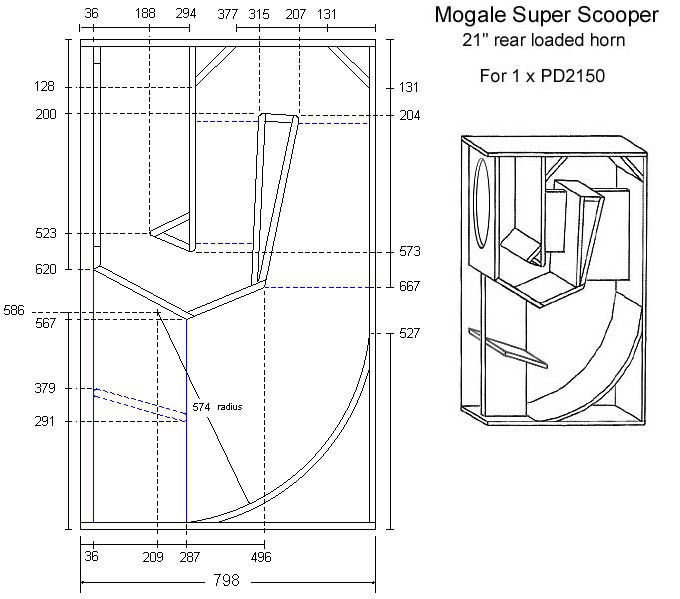
\includegraphics[scale=0.5]{21MogaleSuperScooper.jpg}
    \caption{Vista de perfil del 21" \ Mogale Super Scooper}
    \label{fig:logoETSII}
\end{figure}

En la inmensa mayoría de casos el tamaño original de la imagen no se adapta correctamente a las dimensiones de la página, por lo que es necesario redimensionar la imagen mediante el argumento \texttt{scale} de \textbackslash\texttt{includegraphics}. 

Al igual que para las tablas, existen distintas alternativas en cuanto a su posicionamiento (que, se recuerda, pueden consultarse en \url{https://www.overleaf.com/learn/latex/positioning_images_and_tables}), el título se indica mediante el comando \textbackslash\texttt{caption} y la referencia mediante el comando \textbackslash\texttt{label}. 

Existen, además, diversas opciones en lo relativo al manejo de imágenes que no se detallan en este documento, pero que pueden consultarse en \url{https://es.overleaf.com/learn/latex/Inserting_Images} 

%%%%%%%%%%%%%%%%%%%%%%%%%%%%%%%%%%%%%%%%%%%%%%%%%%


%%%%%%%%%%%%%%%%% - ECUACIONES - %%%%%%%%%%%%%%%%%

\newpage
\section{ECUACIONES} \label{sec:ecuaciones}

Una de las mayores ventajas de \LaTeX \ es lo fácil y rápido que resulta incorporar ecuaciones en el documento. Las ecuaciones se definen en el entorno \texttt{equation}, mediante el cual la identidad de Euler, por ejemplo, quedaría como:

\begin{equation}
    e^{i\pi} + 1 = 0
    \label{eq:euler}
\end{equation}

o la serie de Leibniz:

\begin{equation}
    \sum_{n=0}^\infty \frac{(-1)^n}{2n+1} = \frac{\pi}{4}
    \label{eq:leibniz}
\end{equation}

Como se puede ver, las ecuaciones se numeran de forma automática con respecto al capítulo en el que se encuentran (para no numerar una ecuación basta con definir el entorno como \textbackslash\texttt{begin\{equation*\}}), número al que se puede hacer referencia definiendo el comando \textbackslash\texttt{label}.

En este apartado se utilizan algunos de los símbolos matemáticos básicos, para más información sobre los distintos comandos que corresponden a diversos símbolos puede consultarse \url{https://www.caam.rice.edu/~heinken/latex/symbols.pdf}.


\subsection{Ecuaciones en el texto}

También existe la posibilidad de introducir expresiones matemáticas en una línea de texto encerrando la expresión entre dos símbolos \$, mediante lo cual se puede hacer referencia al número complejo $i$, que puede definirse como $\sqrt{-1}=i$, sin necesidad de interrumpir la oración.


\subsection{Entorno \textbackslash\texttt{split}}

En el caso de que una ecuación sea demasiado larga como para caber en una única línea puede usarse el entorno \texttt{split}, utilizado para el desarrollo de la serie de Taylor de $\sin{x}$ que aparece a continuación:

\begin{equation}
\begin{split}
    \sin{x} = \ & x - \frac{x^3}{3!} + \frac{x^5}{5!} - \frac{x^7}{7!} + \frac{x^9}{9!} - \frac{x^{11}}{11!} + \frac{x^13}{13!} + \dots \\ & + (-1)^n \frac{x^{2n+1}}{(2n+1)!} + \dots \qquad , \forall x \in \mathbb{R}
    \label{eq:taylor}
\end{split}
\end{equation}

La disposición de la ecuación no se hace automáticamente, por lo que es necesario indicar en qué lugar quedan verticalmente alineadas las distintas líneas (esto se realiza mediante el símbolo \& que en este caso va colocado después del $=$ en la primera línea y antes del primer $+$ de la segunda línea) y en qué momento se salta a la línea (que se indica mediante el comando \textbackslash\textbackslash).


\subsection{La herramienta Mathpix}

Mathpix es una aplicación que permite traducir a lenguaje \LaTeX \ cualquier ecuación, ya se encuentre en un archivo PDF o escrita a mano en un folio de papel. Aunque el proceso de plasmar ecuaciones en un documento \LaTeX \ ya es sencillo y rápido, esta herramienta lo vuelve casi instantáneo. La aplicación puede descargarse desde la página web de Mathpix: \url{https://mathpix.com/}.

%%%%%%%%%%%%%%%%%%%%%%%%%%%%%%%%%%%%%%%%%%%%%%%%%%